\chapter{Larutan dan Kelarutan}\label{ch:g6:solutions-and-solubility}

Sebotol air soda dibuka: terdengar desis, dan serbuan gelembung kecil
naik entah dari mana. Sedetik sebelumnya air itu tampak sangat jernih,
padahal selama itu ada gas yang \omterm{def:g2:mixing-and-dissolving:dissolve}{larut} di dalamnya. Padatan \omterm{def:g2:mixing-and-dissolving:dissolve}{larut}, cairan
\omterm{def:g2:mixing-and-dissolving:dissolve}{larut}, dan gas pun \omterm{def:g2:mixing-and-dissolving:dissolve}{larut} --- tetapi tidak pernah tanpa batas. Bab ini
menamai bagian-bagian sebuah larutan dan mengukur berapa banyak suatu
zat yang dapat ditampung sebuah cairan.

\begin{recall}
Padatan yang \omterm{def:g2:mixing-and-dissolving:dissolve}{larut} dalam air hilang dari pandangan dan membiarkan
cairannya jernih; cairan jernih itu adalah larutan, dan zat yang \omterm{def:g2:mixing-and-dissolving:dissolve}{larut}
masih ada di dalamnya (\cref{ch:g2:mixing-and-dissolving}). Larutan
adalah \omterm{def:g6:pure-substances-and-mixtures:homogeneous}{campuran homogen} spesies-spesies kimia
(\cref{ch:g6:pure-substances-and-mixtures}). \omterm{def:g3:separating-mixtures:evaporate}{Menguapkan} airnya
mengembalikan padatan yang \omterm{def:g2:mixing-and-dissolving:dissolve}{larut} (\cref{ch:g3:separating-mixtures}).
\end{recall}

\begin{omfigure}
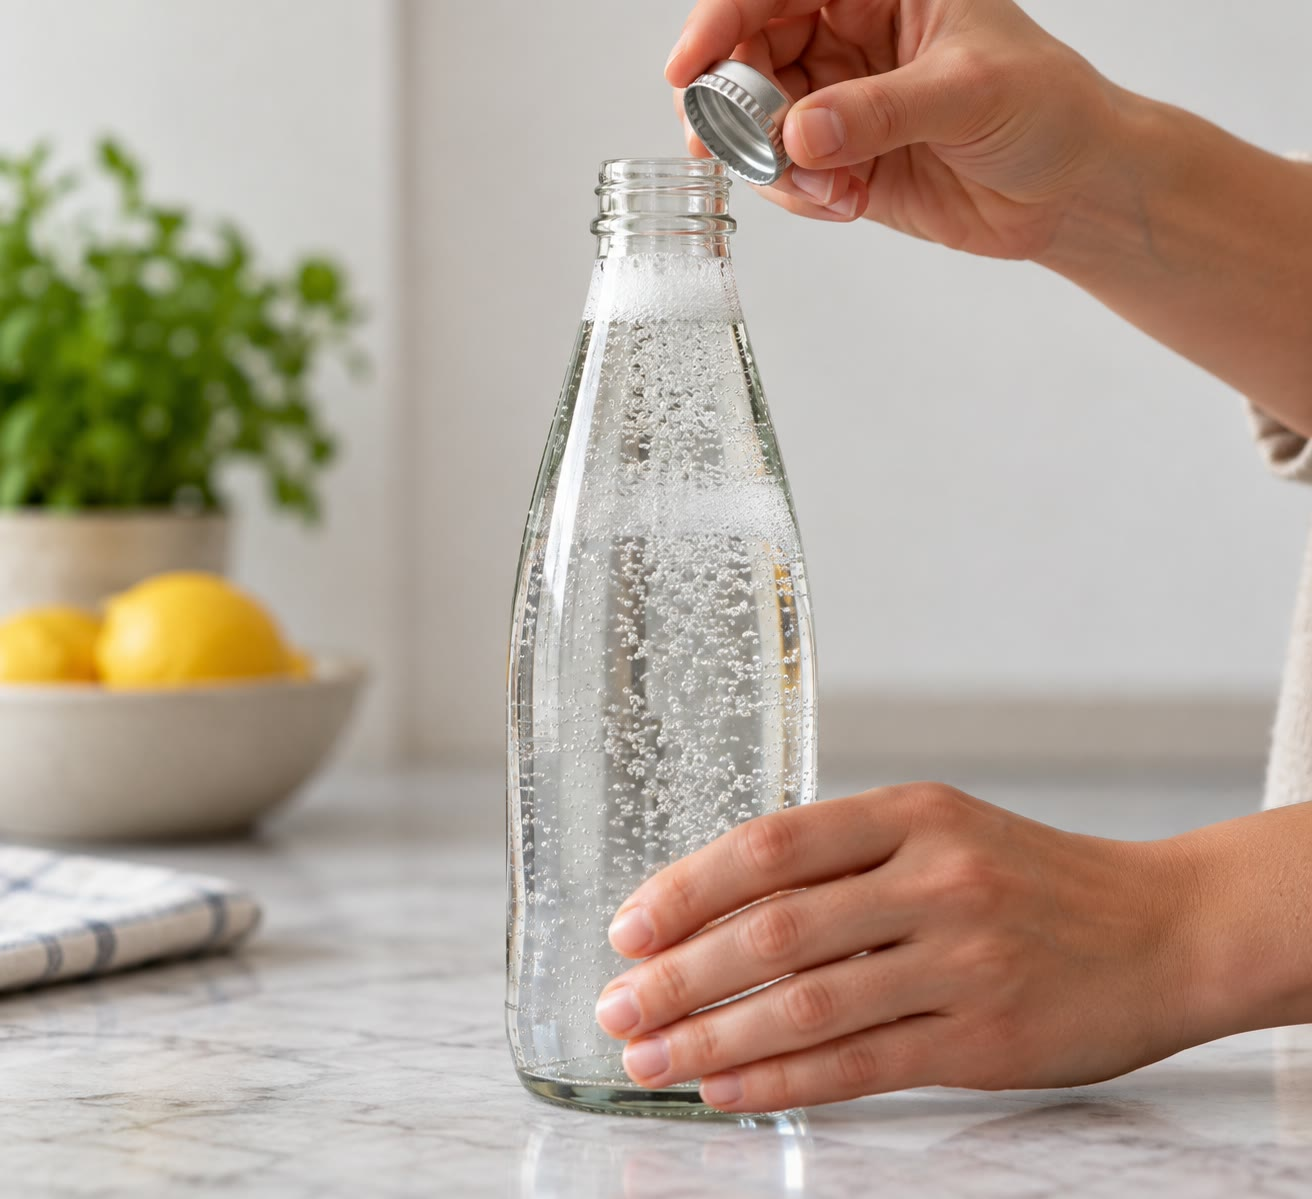
\includegraphics[width=0.5\linewidth]{images/book1/ai/g6-fizzy-water.jpg}

{\small Membuka sebotol air soda: gas yang \omterm{def:g2:mixing-and-dissolving:dissolve}{larut} keluar sebagai
gelembung.}
\end{omfigure}

\section{Zat terlarut dan pelarut}

\begin{definition}[Zat terlarut, pelarut, larutan berair]\label{def:g6:solutions-and-solubility:solute}
Dalam sebuah larutan, zat yang \omterm{def:g2:mixing-and-dissolving:dissolve}{larut} disebut
\emph{zat terlarut}\index{zat terlarut}, dan cairan tempat zat itu
\omterm{def:g2:mixing-and-dissolving:dissolve}{larut} disebut \emph{pelarut}\index{pelarut}. Jika pelarutnya air,
larutan itu disebut \emph{larutan berair}\index{larutan berair}.
\end{definition}

\begin{example}[Pelarut selain air]\label{ex:g6:solutions-and-solubility:solvents}
Air adalah \omterm{def:g6:solutions-and-solubility:solute}{pelarut} yang paling umum, tetapi bukan satu-satunya. Cat
kuku tidak \omterm{def:g2:mixing-and-dissolving:dissolve}{larut} dalam air; cat kuku \omterm{def:g2:mixing-and-dissolving:dissolve}{larut} dalam propanon (aseton),
\omterm{def:g6:solutions-and-solubility:solute}{pelarut} dalam cairan penghapus cat kuku. Gemuk dan cat minyak \omterm{def:g2:mixing-and-dissolving:dissolve}{larut}
dalam tiner. Banyak obat dilarutkan dalam etanol. Sebuah larutan dapat
memiliki beberapa \omterm{def:g6:solutions-and-solubility:solute}{zat terlarut}: air laut mengandung garam terlarut dan
banyak zat lain.
\end{example}

\begin{safety}{\ghs{GHS02}\ghs{GHS07}}
% ledger: ghs:acetone
Propanon (aseton): cairan dan uap yang sangat mudah menyala (GHS02);
menyebabkan iritasi mata dan uapnya dapat menimbulkan kantuk atau
pusing (GHS07). Zat ini dipakai di ruangan yang berventilasi, jauh dari
api.
\end{safety}

\begin{proposition}[Massa-massanya dijumlahkan]\label{prop:g6:solutions-and-solubility:mass}
Massa sebuah larutan sama dengan massa \omterm{def:g6:solutions-and-solubility:solute}{pelarut} ditambah massa \omterm{def:g6:solutions-and-solubility:solute}{zat
terlarut} yang \omterm{def:g2:mixing-and-dissolving:dissolve}{larut}: tidak ada yang hilang ketika sebuah padatan \omterm{def:g2:mixing-and-dissolving:dissolve}{larut},
meskipun padatan itu tidak terlihat lagi.
\end{proposition}

\begin{omfigure}
\begin{tikzpicture}[font=\small, scale=1.15]
  \pic[transform shape] at (0,0) {balance};
  \pic[transform shape] at (0,0.8) {beaker={0.5}{omWater!80}};
  \node[anchor=north, align=center] at (0,-0.1) {\qty{100}{g} air};
  \node at (1.85,1.3) {$+$};
  \pic[transform shape] at (3.5,0) {balance};
  \fill[white, draw=black!45] (3.0,0.8) rectangle (4.0,0.9);
  \fill[white, draw=black!45] (3.15,0.9) -- (3.85,0.9) -- (3.5,1.2) -- cycle;
  \node[anchor=north, align=center] at (3.5,-0.1) {\qty{10}{g} gula};
  \draw[->, thick, omProp] (4.9,1.2) -- (6.0,1.2) node[midway, above, text=black]
    {aduk};
  \pic[transform shape] at (7.4,0) {balance};
  \pic[transform shape] at (7.4,0.8) {beaker={0.52}{omWater!80}};
  \node[anchor=north, align=center] at (7.4,-0.1) {\qty{110}{g} air gula};
\end{tikzpicture}

{\small Melarutkan \qty{10}{g} gula dalam \qty{100}{g} air menghasilkan
\qty{110}{g} larutan (massa gelas kimianya tidak dihitung).}
\end{omfigure}

\section{Kejenuhan dan kelarutan}

\begin{definition}[Larutan jenuh]\label{def:g6:solutions-and-solubility:saturated}
Sebuah larutan disebut \emph{larutan jenuh}\index{larutan jenuh} jika
larutan itu tidak dapat melarutkan lagi \omterm{def:g6:solutions-and-solubility:solute}{zat terlarutnya}: \omterm{def:g6:solutions-and-solubility:solute}{zat terlarut}
yang ditambahkan tetap berada di dasar, tidak \omterm{def:g2:mixing-and-dissolving:dissolve}{larut}, selama apa pun kita
mengaduk.
\end{definition}

\begin{definition}[Kelarutan]\label{def:g6:solutions-and-solubility:solubility}
Yang disebut \emph{kelarutan}\index{kelarutan} suatu \omterm{def:g6:solutions-and-solubility:solute}{zat terlarut} dalam
suatu \omterm{def:g6:solutions-and-solubility:solute}{pelarut} adalah massa \omterm{def:g6:solutions-and-solubility:solute}{zat terlarut} terbesar yang dapat dilarutkan
oleh sejumlah tertentu \omterm{def:g6:solutions-and-solubility:solute}{pelarut}, pada suhu tertentu. Untuk padatan dalam
air, kelarutan sering dinyatakan dalam gram per liter (atau per
kilogram) air.
\end{definition}

\begin{proposition}[Beberapa kelarutan dalam air]\label{prop:g6:solutions-and-solubility:values}
% ledger: sol:NaCl, sol:sucrose, sol:CO2, sol:O2 (O2: 31 mL/L, 31/24.0 x 32 = 0.041 g/L at 20 C)
\omterm{def:g6:solutions-and-solubility:solubility}{Kelarutan} dalam air yang terukur sangat berbeda-beda:
\begin{center}
\small
\begin{tabular}{lll}
\hline
\omterm{def:g6:solutions-and-solubility:solute}{zat terlarut} & \omterm{def:g6:solutions-and-solubility:solubility}{kelarutan} dalam air & kondisi \\
\hline
gula (sukrosa) & sekitar \qty{2000}{g} per liter air & suhu kamar \\
garam (natrium klorida) & \qty{360}{g} per kilogram air & \qty{25}{\celsius} \\
karbon dioksida & sekitar \qty{1.5}{g} per liter & \qty{25}{\celsius}, di bawah gasnya \\
oksigen & sekitar \qty{0.04}{g} per liter & \qty{20}{\celsius}, di bawah gasnya \\
pasir, kapur tulis & praktis tidak ada & --- \\
\hline
\end{tabular}
\end{center}
Seliter air dapat melarutkan gula yang lebih berat daripada air itu
sendiri, tetapi oksigen setengah gram pun tidak.
\end{proposition}

\begin{method}[Akankah semuanya larut?]\label{met:g6:solutions-and-solubility:will-it}
Untuk mengetahui apakah \omterm{def:g6:solutions-and-solubility:solute}{zat terlarut} bermassa $m$ \omterm{def:g2:mixing-and-dissolving:dissolve}{larut} seluruhnya dalam
sejumlah volume air:
\begin{enumerate}
  \item carilah \omterm{def:g6:solutions-and-solubility:solubility}{kelarutan} \omterm{def:g6:solutions-and-solubility:solute}{zat terlarut} itu (dalam g per liter air);
  \item hitung massa terbesar yang dapat dilarutkan oleh volume air itu;
  \item bandingkan dengan $m$: jika $m$ lebih kecil, semuanya \omterm{def:g2:mixing-and-dissolving:dissolve}{larut}; jika
        $m$ lebih besar, larutannya jenuh dan sisanya tetap berada di
        dasar.
\end{enumerate}
\end{method}

\begin{example}[Garam dalam segelas air]\label{ex:g6:solutions-and-solubility:glass}
% ledger: sol:NaCl
Dapatkah \qty{50}{g} garam \omterm{def:g2:mixing-and-dissolving:dissolve}{larut} dalam \qty{200}{mL} air (sekitar
\qty{200}{g})? Satu kilogram air melarutkan paling banyak \qty{360}{g}
garam, jadi \qty{200}{g} air melarutkan paling banyak $360 \times
\frac{200}{1000} = \qty{72}{g}$. Karena $50 < 72$, semua garam itu
\omterm{def:g2:mixing-and-dissolving:dissolve}{larut}.
\end{example}

\begin{omfigure}
\begin{tikzpicture}[font=\small, scale=1.15]
  \pic[transform shape] at (0,0) {beaker={0.6}{omWater!80}};
  \node[anchor=north, align=center] at (0,-0.15) {sedikit garam:\\ larut semua};
  \pic[transform shape] at (3.2,0) {beaker={0.6}{omWater!80}};
  \node[anchor=north, align=center] at (3.2,-0.15) {lebih banyak garam:\\ tepat jenuh};
  \pic[transform shape] at (6.4,0) {beaker={0.6}{omWater!80}};
  \fill[black!12, draw=black!50] (5.7,0) -- (7.1,0) -- (6.9,0.2) -- (5.9,0.2) -- cycle;
  \foreach \x in {5.85,6.05,6.25,6.45,6.65,6.85} \fill[black!45] (\x,0.09) circle (0.03);
  \node[anchor=north, align=center] at (6.4,-0.15) {garam terlalu banyak:\\ sisanya tidak larut};
\end{tikzpicture}

{\small Menambahkan garam makin banyak ke dalam air yang sama. Begitu
larutannya jenuh, garam tambahan tetap berada di dasar.}
\end{omfigure}

\begin{inthelab}[Menjenuhkan air garam]
Guru menambahkan garam ke dalam \qty{100}{mL} air sesendok demi
sesendok, sambil mengaduk dengan baik setiap kali. Sendok-sendok
pertama menghilang; lalu satu sendok tidak \omterm{def:g2:mixing-and-dissolving:dissolve}{larut} seluruhnya lagi dan
butiran putih tetap berada di dasar: larutannya jenuh. Penimbangan
garam yang dipakai menunjukkan bahwa sekitar \qty{36}{g} telah \omterm{def:g2:mixing-and-dissolving:dissolve}{larut}.
\end{inthelab}

\section{Cairan yang dapat bercampur dan yang tidak}

\begin{definition}[Cairan yang dapat bercampur dan yang tidak]\label{def:g6:solutions-and-solubility:miscible}
Dua cairan disebut \emph{dapat bercampur}\index{dapat bercampur} jika,
setelah \omterm{def:g2:mixing-and-dissolving:mix}{dicampur}, keduanya membentuk satu cairan homogen. Keduanya
disebut \emph{tidak dapat bercampur}\index{tidak dapat bercampur} jika
keduanya memisah menjadi dua lapisan, dengan yang lebih ringan di atas.
\end{definition}

\begin{example}[Air dengan etanol, air dengan minyak]\label{ex:g6:solutions-and-solubility:liquids}
Air dan etanol \omterm{def:g6:solutions-and-solubility:miscible}{dapat bercampur}: setelah dikocok bersama, keduanya
membentuk satu cairan jernih. Air dan minyak \omterm{def:g6:solutions-and-solubility:miscible}{tidak dapat bercampur}:
sekuat apa pun dikocok, minyak naik kembali dan terapung di atas air
sebagai lapisan tersendiri. Dalam stoples saus salad, minyak terapung di
atas cuka, yang sebagian besar berupa air.
\end{example}

\begin{omfigure}
\begin{tikzpicture}[font=\small, scale=1.3]
  \pic[transform shape] at (0,0) {testtube={0.6}{omWater!80}};
  \node[anchor=north, align=center] at (0,-0.15) {air + etanol:\\ satu lapisan};
  \pic[transform shape] at (3,0) {testtube={0.65}{yellow!55!orange!60}};
  \begin{scope}
    \clip (2.75,3) -- (2.75,0.25) arc[start angle=180, end angle=360, radius=0.25]
      -- (3.25,3) -- cycle;
    \fill[omWater!80] (2.7,0) rectangle (3.3,1.1);
  \end{scope}
  \draw[omGlass, line width=0.7pt] (2.75,3) -- (2.75,0.25) arc[start angle=180,
    end angle=360, radius=0.25] -- (3.25,3);
  \draw[<-, omProp, thick] (3.3,1.55) -- (4.1,1.75) node[right, text=black] {minyak};
  \draw[<-, omProp, thick] (3.3,0.6) -- (4.1,0.6) node[right, text=black] {air};
  \node[anchor=north, align=center] at (3,-0.15) {air + minyak:\\ dua lapisan};
\end{tikzpicture}

{\small Cairan yang \omterm{def:g6:solutions-and-solubility:miscible}{dapat bercampur} membentuk satu lapisan; cairan yang
\omterm{def:g6:solutions-and-solubility:miscible}{tidak dapat bercampur} membentuk dua.}
\end{omfigure}

\begin{omfigure}
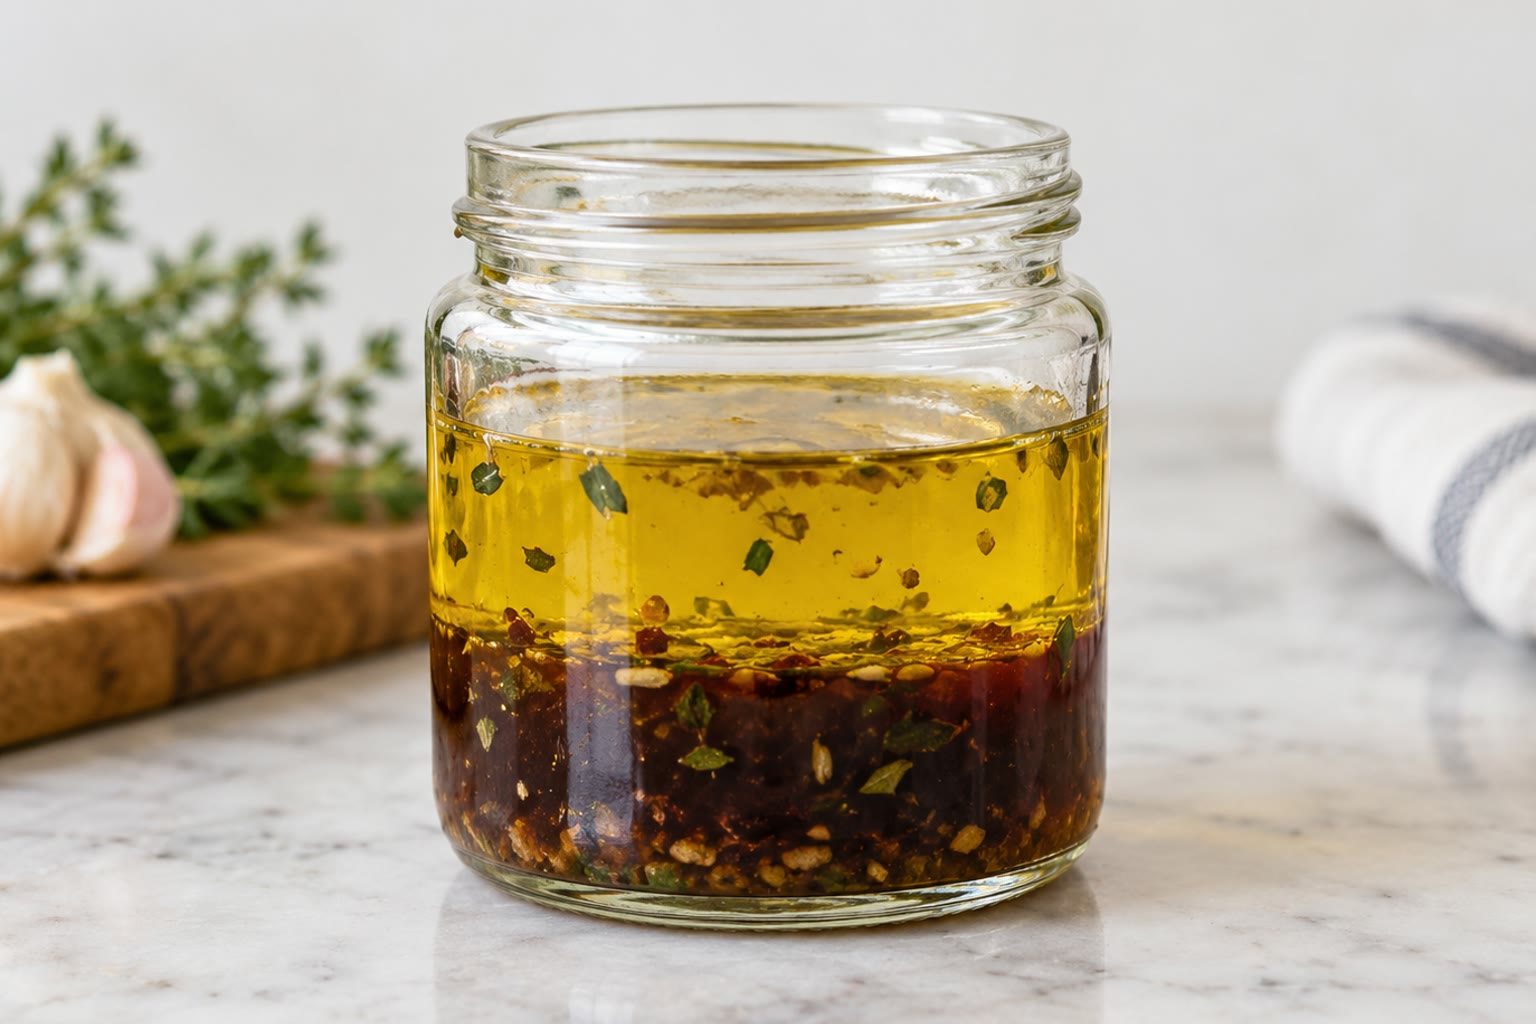
\includegraphics[width=0.45\linewidth]{images/book1/ai/g6-vinaigrette.jpg}

{\small Saus salad: minyak dan cuka \omterm{def:g6:solutions-and-solubility:miscible}{tidak dapat bercampur}.}
\end{omfigure}

\section{Gas pun larut}

\begin{proposition}[Gas yang larut]\label{prop:g6:solutions-and-solubility:gases}
Gas \omterm{def:g2:mixing-and-dissolving:dissolve}{larut} dalam air, sedikit. Minuman bersoda dibuat dengan melarutkan
karbon dioksida ke dalamnya di bawah tekanan dalam botol tertutup;
ketika botol dibuka, sebagian gas keluar kembali sebagai gelembung. Air
yang bersentuhan dengan \omterm{def:g4:air-a-mixture-of-gases:air}{udara} mengandung sedikit oksigen terlarut, yang
diambil ikan melalui insangnya. Gas lebih sedikit \omterm{def:g2:mixing-and-dissolving:dissolve}{larut} dalam air hangat
daripada dalam air dingin: minuman bersoda yang hangat lebih cepat
kehilangan sodanya.
\end{proposition}

\begin{example}[Samudra dan karbon dioksida]\label{ex:g6:solutions-and-solubility:oceans}
Samudra bersentuhan dengan \omterm{def:g4:air-a-mixture-of-gases:air}{udara} di atas dua pertiga permukaan Bumi.
Karbon dioksida dari \omterm{def:g4:air-a-mixture-of-gases:air}{udara} \omterm{def:g2:mixing-and-dissolving:dissolve}{larut} di dalamnya, sehingga samudra menyerap
sebagian karbon dioksida yang dilepaskan manusia ke \omterm{def:g4:air-a-mixture-of-gases:air}{udara}.
\end{example}

\begin{omfigure}
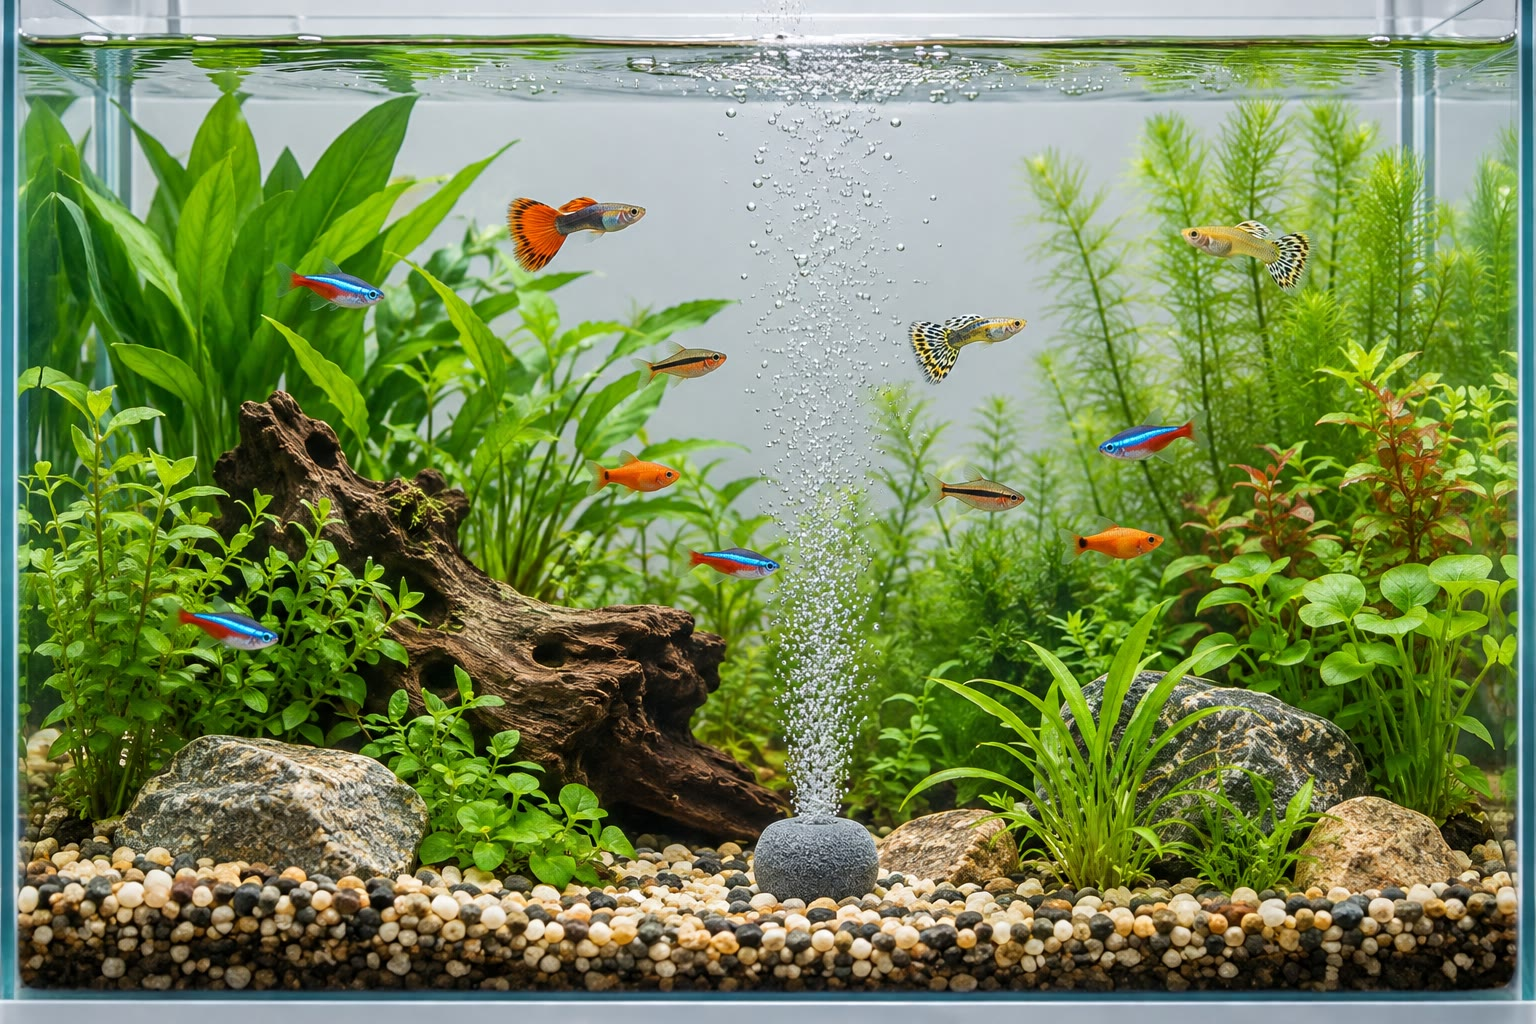
\includegraphics[width=0.5\linewidth]{images/book1/ai/g6-fish-tank.jpg}

{\small Akuarium: gelembung \omterm{def:g4:air-a-mixture-of-gases:air}{udara} menjaga agar air tetap mengandung
oksigen terlarut untuk ikan-ikan.}
\end{omfigure}

\section{Latihan}

\begin{exercise}[$\star$]\label{exo:g6:solutions-and-solubility:1}
Dalam air gula, sebutkan \omterm{def:g6:solutions-and-solubility:solute}{zat terlarut} dan \omterm{def:g6:solutions-and-solubility:solute}{pelarutnya}. Apakah air gula
itu \omterm{def:g6:solutions-and-solubility:solute}{larutan berair}?
\end{exercise}

\begin{exercise}[$\star$]\label{exo:g6:solutions-and-solubility:2}
Apa itu \omterm{def:g6:solutions-and-solubility:saturated}{larutan jenuh}? Bagaimana kamu dapat melihat bahwa sebuah larutan
sudah jenuh?
\end{exercise}

\begin{exercise}[$\star$]\label{exo:g6:solutions-and-solubility:3}
\qty{20}{g} garam dilarutkan dalam \qty{250}{g} air. Berapa massa
larutannya?
\end{exercise}

\begin{exercise}[$\star$]\label{exo:g6:solutions-and-solubility:4}
\omterm{def:g6:solutions-and-solubility:miscible}{Dapat bercampur} atau tidak dengan air: etanol, minyak goreng, cuka?
\end{exercise}

\begin{exercise}[$\star$]\label{exo:g6:solutions-and-solubility:5}
Sebutkan \omterm{def:g6:solutions-and-solubility:solute}{pelarut} dalam cairan penghapus cat kuku dan jelaskan arti
kedua piktogramnya.
\end{exercise}

\begin{exercise}[$\star\star$]\label{exo:g6:solutions-and-solubility:6}
Dengan \omterm{def:g6:solutions-and-solubility:solubility}{kelarutan} garam, tentukan massa garam terbesar yang dapat
dilarutkan oleh \qty{500}{g} air pada \qty{25}{\celsius}.
\end{exercise}

\begin{exercise}[$\star\star$]\label{exo:g6:solutions-and-solubility:7}
\qty{80}{g} garam diaduk ke dalam \qty{200}{g} air pada
\qty{25}{\celsius}. Apakah semuanya \omterm{def:g2:mixing-and-dissolving:dissolve}{larut}? Jika tidak, berapa massa
yang tertinggal di dasar?
\end{exercise}

\begin{exercise}[$\star\star$]\label{exo:g6:solutions-and-solubility:8}
\qty{25}{g} gula dilarutkan dalam \qty{225}{g} air. Berapa persen
massa larutan itu yang berupa gula?
\end{exercise}

\begin{exercise}[$\star\star$]\label{exo:g6:solutions-and-solubility:9}
Lihatlah gambar tiga gelas kimia berisi air garam. Di gelas kimia mana
garam masih dapat \omterm{def:g2:mixing-and-dissolving:dissolve}{larut} lagi?
\end{exercise}

\begin{exercise}[$\star\star$]\label{exo:g6:solutions-and-solubility:10}
Mengapa sebotol air soda berdesis ketika dibuka, dan tidak sebelumnya?
\end{exercise}

\begin{exercise}[$\star\star\star$]\label{exo:g6:solutions-and-solubility:11}
Seliter air dapat melarutkan sekitar \qty{2000}{g} gula tetapi hanya
sekitar \qty{0.04}{g} oksigen. Berapa kali lebih banyak gula itu
dibandingkan oksigen?
\end{exercise}

\begin{exercise}[$\star\star\star$]\label{exo:g6:solutions-and-solubility:12}
Pada musim panas, air kolam menjadi hangat dan ikan-ikan naik ke
permukaan untuk menghirup \omterm{def:g4:air-a-mixture-of-gases:air}{udara}. Pakailah bab ini untuk menjelaskan
mengapa.
\end{exercise}

\section{Soal: Air Garam Pembuat Keju}

\begin{problem}[{Soal akhir pekan --- bak air garam jenuh untuk keju, dan
apa yang dilakukan panas musim panas terhadapnya}]
\label{pb:g6:solutions-and-solubility:1}
% ledger: sol:NaCl (360 g per kg of water; 1 L of water taken as 1 kg)
Banyak keju direndam beberapa jam dalam bak air garam: air yang jenuh
garam. Seorang pembuat keju mengisi sebuah bak dengan \qty{20}{L} air
(\qty{20}{kg}) dan menambahkan garam sampai ada sebagian yang tetap tidak
\omterm{def:g2:mixing-and-dissolving:dissolve}{larut} di dasar. Anggaplah \omterm{def:g6:solutions-and-solubility:solubility}{kelarutan} garam \qty{360}{g} per kilogram
air.

\medskip
\noindent\textbf{Bagian I --- Istilah.}
\begin{enumerate}
  \item Dalam air garam itu, mana \omterm{def:g6:solutions-and-solubility:solute}{zat terlarut} dan mana \omterm{def:g6:solutions-and-solubility:solute}{pelarutnya}?
  \item Apa arti ``jenuh'' bagi air garam itu?
  \item Mengapa pembuat keju menambahkan garam sampai sedikit tertinggal
        di dasar?
\end{enumerate}

\medskip
\noindent\textbf{Bagian II --- Membuat air garam.}
\begin{enumerate}[resume]
  \item Berapa massa garam yang \omterm{def:g2:mixing-and-dissolving:dissolve}{larut} dalam \qty{20}{kg} air itu?
  \item Berapa massa air garamnya (tanpa garam yang tidak \omterm{def:g2:mixing-and-dissolving:dissolve}{larut})?
  \item Berapa persen massa air garam itu yang berupa garam? Bulatkan ke
        bilangan bulat terdekat.
  \item Suatu hari hanya \qty{5}{kg} garam yang ditambahkan. Apakah air
        garam itu jenuh? Berapa banyak garam lagi yang masih dapat
        dilarutkannya?
\end{enumerate}

\medskip
\noindent\textbf{Bagian III --- Musim panas yang terik.}
Selama satu minggu yang panas, \qty{5}{L} (\qty{5}{kg}) air \omterm{def:g3:separating-mixtures:evaporate}{menguap} dari
air garam jenuh pada Bagian II, dan tidak ada garam yang hilang.
\begin{enumerate}[resume]
  \item Berapa banyak air yang tersisa di dalam bak?
  \item Berapa massa garam yang masih dapat dilarutkan oleh air ini?
  \item Apa yang terjadi pada garam yang tidak dapat ditampung lagi oleh
        air yang tersisa?
  \item Bagaimana pembuat keju dapat melihat, dengan mata, bahwa hal itu
        telah terjadi?
  \item Hitung massa garam yang telah mengkristal di dasar bak.
\end{enumerate}
\end{problem}
